\section{Server Configuration for Scan Agents}\label{sec:scan-agent-server}

Implementing the Scan Agents requires an AMQP message queue server that
is used for communication between the \cxoneflow server and the Scan
Agents.  Details about the message queue deployment can be found in Section \ref{sec:external-mq}.

The examples in this section show a configuration that uses environments names as tags to
instruct the Scan Agents with that environment tag to perform pre-scan and \scaresolver
execution.  The tags names can be used to establish the Scan Agent affinity with \cxone projects
in whatever way fits your organization best.

\subsection{\cxoneflowtext\space Endpoint Configuration}

The \cxoneflow endpoint server \intlink{sec:yaml-config}{YAML configuration} will not utilize Scan Agents
by default.  Using Scan Agents requires a public/private key pair; the private key is configured
for use on the \cxoneflow endpoint and the public key is installed with each Scan Agent.  Before
configuring the use of Scan Agents, it is recommended to read about the security
concepts in Section \ref{sec:scan-agent-security}.

The \cxoneflow endpoint will send messages signed by the private key to the Scan
Agents using the message queue.  The receiving Scan Agent will validate the signature
using the public key; if the signature is not valid, the Scan Agent will reject the message
and perform no actions.

Scan Agents are identified using agent tags.  The \cxoneflow endpoint is configured by the
administrator with a list of allowed tags to prevent arbitrary Scan Agents from requesting
scan activity delegation.  The server-side tag configuration is also used to set up the communication
with Scan Agents via the message queue.  Anyone who installs a Scan Agent must configure it to respond to messages
targeting at least one valid Scan Agent tag.


\subsubsection{Generating a Public/Private Key Pair}\label{ref:server-key-pair}

There are many ways to generate a public/private key pair.  There are only a few requirements
for key pairs produced by any method:

\begin{itemize}
  \item The private key must be unencrypted.
  \item Both the private and public key files must be PEM encoded.
  \item The public/private key algorithm is supported by the install Python \texttt{cryptography} library.
    As of this release, these algorithms have been tested:
  \begin{itemize}
      \item RSA 4096-bit
      \item ECDSA secp256k1
  \end{itemize}
\end{itemize}

One easy method of generating a public/private key pair is to use OpenSSL.  To generate an ECDSA public/private key pair,
the following command can be used.  The command will create the file \texttt{ec-priv.pem} that holds the unencrypted private key
and the file \texttt{ec-pub.pem} that holds the public key.

\begin{code}{OpenSSL Public/Private Key Creation}{[ECDSA]}{}
openssl ecparam -name secp256k1 -genkey -noout | tee ec-priv.pem | openssl ec -pubout > ec-pub.pem  
\end{code}

To generate an RSA 4096-bit public/private key pair,
the following command can be used.  The command will create the file \texttt{rsa-priv.pem} that holds the unencrypted private key
and the file \texttt{rsa-pub.pem} that holds the public key.

\begin{code}{OpenSSL Public/Private Key Creation}{[RSA]}{}
openssl genrsa 4096 |tee rsa-priv.pem | openssl rsa -pubout > rsa-pub.pem
\end{code}

The private key file may be stored as a secret referenced in the configuration YAML element \intlink{sec:yaml-resolver-private-key}{resolver->private-key}.

\subsubsection{Scan Agent YAML Configuration}\label{sec:scan-agent-yaml-config}
Figure \ref{fig:scan-agent-config-yaml} shows the common YAML configuration for resolver agents with a list of allowed tags.
This YAML configuration is provided in the configuration example artifacts that can be downloaded from the \cxoneflow release
artifacts.

Some of the things to note in these examples:

\begin{itemize}
  \item The AMQP URL is stored as a secret since it contains credentials.
  \item The AMQP connection is common in both the \texttt{feedback} and \texttt{resolver} configuration.
  This configuration allows the feedback workflows and Scan Agent workflows to use the same external message queue.
  \item The Scan Agent configuration is often easily maintained as a common configuration that is applied to 
  all service definitions for all SCM types.  
\end{itemize}


\begin{figure}[h]
    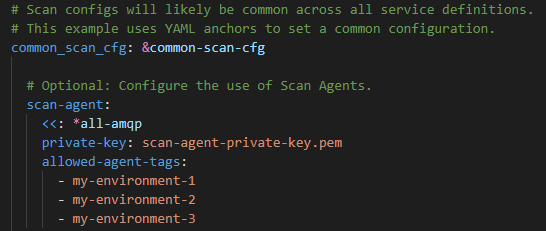
\includegraphics[scale=1]{graphics/scan-agent-config-yaml.png}
    \centering
    \caption{Scan Agent Common Configuration for Server YAML}
    \label{fig:scan-agent-config-yaml}
\end{figure}


\subsection{Message Queue Configuration}

The \cxoneflow endpoint will configure the AMQP Exchanges and Queues upon start.  Adding any
allowed Scan Agent tags will require at least one \cxoneflow endpoint restart so that the
appropriate message queue elements for that tag can be constructed.

The message queue connection credentials for the \cxoneflow endpoint will have the 
permissions required to enable configuring the message queue elements.  Section \ref{sec:external-mq}
will give more details about the appropriate message queue user permissions for the \cxoneflow endpoint.

Configuring a Scan Agent will require each agent to have credentials that allow limited
access to the message queue.  Section \ref{sec:scan-agent-security} has more details about the
authorization that should be assigned to credentials used by Scan Agents.

The YAML examples in \intlink{sec:scan-agent-yaml-config}{the previous section} demonstrated the use of a single
message queue instance for both the communication with the Scan Agents and feedback workflow
orchestration.  While using a single message queue may make the \cxoneflow configuration simpler, it is not
strictly required to use the same message queue connection for all configurations.  Each configuration can
use a segregated message queue server if this is desired.  This segregation includes the use
of \extlink{https://www.rabbitmq.com/docs/vhosts}{virtual hosts} if supported by the AMQP endpoint server.


\subsection{Deployment Considerations}

The YAML examples in \intlink{sec:scan-agent-yaml-config}{Scan Agent configuration section} demonstrated agent tags
configured in a single endpoint service definition.  The allowed tags in each service endpoint are
indicating which agent tags can execute resolver scans and pre-scan scripts for an event handled by that service endpoint.
The tags are used to communicate with Scan Agents that listen for messages directed to that agent tag and
have the public key associated with the private key defined in the service configuration.

The important thing to note is that Scan Agents are not tied to a single
\cxoneflow endpoint service definition.  The Scan Agents will typically have
tooling and configuration that can be used for any code that requires that tooling.  This
has some implications in how Scan Agents can be deployed:

\begin{itemize}
  \item One instance of a Scan Agent can handle multiple tags.
  
  \item More than one instance of a Scan Agent can be deployed to handle the same tag.  This increases the number of concurrently
  executing Scan Agents.

  \item The Scan Agent tag/private key pair can be different in each service definition.  It is recommended to
  use duplicate Scan Agent tags across \cxoneflow service definitions only when those tags all share the same public/private
  key pair.

  \item Not all service definitions need to support the same allowed Scan Agent tags.  If there are Scan Agents
  that should only be used by a specific service definition, it is recommended to use the allowed Scan Agent tag list
  in combination with Scan Agent connection credentials that limit the agent's ability to receive
  communications for specific tags.

  \item For complex \cxoneflow configurations that have many service definitions, it is recommended to engineer
  deployment of Scan Agents to be as simple as possible.
    
\end{itemize}


